\documentclass{report}
\usepackage{graphicx} % Required for inserting images
\usepackage{amsmath, amssymb, amsthm, mathrsfs, derivative}
\usepackage[swedish]{babel}
\usepackage[
	top=0.5cm,
	left=1.0cm,
	right=1.0cm,
	bottom=0.5cm
]{geometry}
\usepackage{enumitem}
\newcommand{\hidden}[1]{}
\usepackage{xcolor}
\usepackage{hyperref}
\usepackage{booktabs}
\usepackage{float}

\newcommand{\timage}[2]{$\vcenter{\hbox{\includegraphics[width=#1\linewidth]{#2}}}$}
\title{ME1317 Artiklar}
\author{Alexander Järvheden}
\date{April 2026}

\usepackage{tikz}
\usepackage{eso-pic}
\usepackage{comment}

\usetikzlibrary{calc}

% Kommentera bort \iffalse \fi blocket

\begin{comment}
\AddToShipoutPictureBG{

\begin{tikzpicture}[remember picture,overlay]\foreach \i in {1,...,8} { \draw[black!100] ($(current page.south west)+(0,\i*\paperheight/8)$) -- ($(current page.south east)+(0,\i*\paperheight/8)$); }\end{tikzpicture} }
\end{comment}
\begin{document}
	\maketitle
	\chapter{Kontrollskrivning 1}
	\begin{table}[ht!]
		\centering
		\Large
		\begin{tabular}{c|c}
			\toprule Artikel     & Backtest result \\
			\midrule Barry et al & alla fel        \\
			Saragih et al        & alla rätt
		\end{tabular}
	\end{table}

	\newpage
	\section{Barry, M., T. Dundon, A. Wilkinson (2018) -- Employee
	Voice}
	\textbf{Stupidity management} är när ledningen förhindrar
	anställda att uttrycka en kritisk röst, i sin tur leder till
	sämre decision-making och kommunikation. \textbf{Hirschman
	(1970)} definierar röst som ett försök att förändra istället
	för att eskapera en situation. \textbf{double-breasting
	voice} är när management restrukturerar organisationen på så
	sett att organisationen är både innanför och utanför fackföreningen

	\textbf{OB röst} bygger på antagande om likriktning mellan managment
	och anställdas motiv för röst. De anställda är motiverade
	att uttrycka röst för att förbättra organisationen, och management
	är motiverade att lyssna på röst för att förbättra organisationen.
	Även \textbf{klagomål} är en form av OB röst eftersom klagomål
	är ett motiv att yttra sig för att förbättra organisationen.
	\textbf{Röst} ses som en frivillig individuell handling av anställda
	snarare än en kollektiv handling. Rösten är oftast
	informell istället för institutionell. Några \textbf{utlösare}
	av röst är bl.a. personliga egenskaper, ledarskapsstil, upplevd
	organisatorisk öppen- och mottaglighet samt trygghet att
	röst inte leder till vedergällning. Skillnaden mellan \textbf{OB-}
	och \textbf{ER} röst är att OB lägger tonvikt på de individuella
	informella utlösare av röst, medans ERs fokus ligger på
	formella kollektiva utlösare av röst.

	\textbf{HRM röst} bygger på paradigmen att låta anställa påverka
	organisatoriska beslut leder till bättre beslut och mer förståelse.
	HRM lägger förenat med \textbf{HPWS (High Performance Work Systems)}
	vars syfte är att förse arbete som är berikande för anställda
	som i sin tur gör att anställda är villig att delta mer i alla
	aspekter av arbetet. En \textbf{kritik mot HPWS} är att kostnaden
	för att implementera HPWS är hög och det är svårt att mäta hur
	stor nyttan är. Både \textbf{HRM} och \textbf{OB}
	perspektivet delar många likheter som fokus på hur
	managment kan främja röst. Det finns \textbf{tre}
	huvudsakliga komponenter för \textbf{direkt röst} inom \textbf{HR
	perspektivet}: \textit{1) Hög autonomiska arbetsuppgifter 2)
	Autonoma organisationsstrukturer 3) Direkta kommunikationsvägar
	med ledningen.} \textbf{Anställdas röst} ses som ett alternativ
	för exit (sorti).

	\textbf{ER röst} bygger på antagande att anställda är
	egenintressen skilt från organisationens intressen. Ser \textbf{kollektiva
	strukturer} såsom fackföreningar, lagar och regler som utlösare
	för anställdas röst. En \textbf{skillnad} mellan \textbf{ER}
	och \textbf{OB} perspektivet är att \textbf{ER} lägger
	högre vikt på kontext, med kontext menas exempelvis vilken arbetsuppgifter,
	intellektuellt krav på arbete, huruvida fackföreningar finns
	närvarande, etc. \textbf{OB} lägger högre vikt på
	individuella faktorer i.e. personlighet och lednings mottaglighet.
	Arbete som känntecknas av \textbf{hög intelligens och
	koordination} tenderar även ha högre engagemang av \textbf{anställdas
	röst} röst

	\textbf{LPT röst} har en mer restriktiv syn angående i
	vilken utsträckning anställda kan motsätta anställdas
	intressen. \textbf{LPT} ser röst som en brygga mellan
	arbetsplatskonflikter och större macroekonomiska problem. \textbf{LPT}
	beskriver även \textbf{Cycle theory} som säger att arbetsgivare
	växlar mellan att erbjuda inflytande/deltagande och att ta bort
	det, beroende på hur hotade de känner sig av den fackliga
	organisationen.\textit{Hot = mer inflytande. Inget hot = mindre
	inflytande.} Sammanfattningsvis har \textbf{LPT} en mer
	kritisk syn på rösten och ställer sig kritik för
	antaganden om ömsesidig nytta. \textbf{LPT} tar även ett
	macro perspektiv bort från individen och fokuserar på
	institutioner och sociopolitiska perspektiv. \textbf{En
	kritik} mot \textbf{LPT} är att perspektivet ignorerar pro-sociala
	aspekter av rösten och betraktar arbete från en kritiskt perspektiv.

	\textbf{Integrerande perspektiv} studier om anställdas
	röst präglas av några akademiska dogmer med överlapp
	mellan vissa perspektiv. \textbf{OB} och \textbf{HRM} anser
	att the finns ett "business case" for anställdas röst och antar
	att anställda och arbetsgivare är liktriktade. \textbf{ER} och
	\textbf{LPT} ser röst som en utmaning mot arbetsgivarens
	makt medans \textbf{OB} inte alls ser röst som en utmaning.
	\textbf{ER} anser att anställda har andra intressen än arbetsgivaren
	röst är ett sätt att uttrycka anställdas intressen snarare än
	att förbättra organisationen, \textbf{ER} är även mer intresserad
	av institutionella faktorer istället för individuella faktorer.
	\begin{figure}[H]
		\centering
		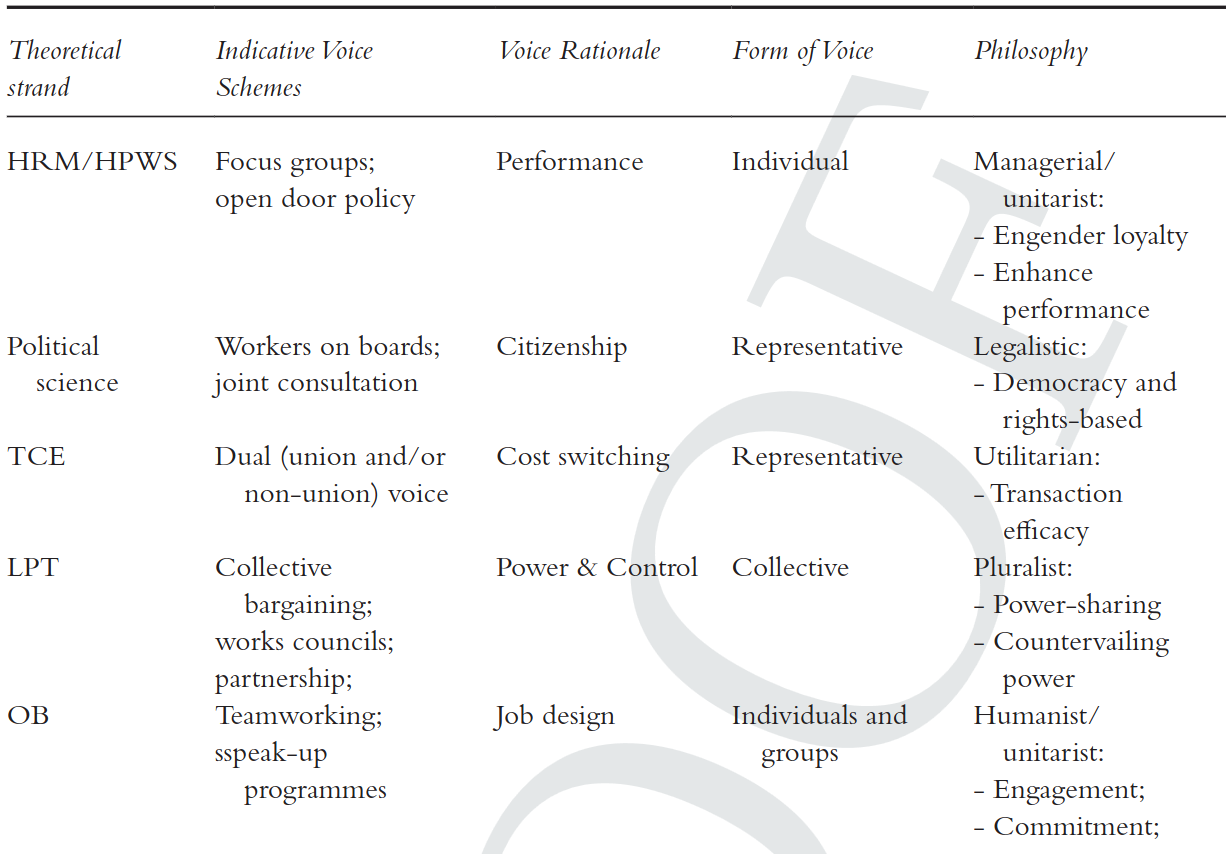
\includegraphics[width=0.55\textwidth]{
			VoicePerspectives.png
		}
	\end{figure}
	Analyser av utlösare för anställdas röst beror på
	anställdas motiv för röst. \textbf{Motivet} kan vara: förbättra
	företaget, begränsa arbetsgivarens makt och rättvisa
	orienterad (whistleblowing). Röst kan vara \textbf{Pro-social}
	och inte \textbf{Pro-social} samtidigt. En individ kan
	föreslå en förbättring till ledningen som är en pro-social
	handling men i själva verket är motivet att själv klättra
	i karriären. \textbf{Makt och röst:} \textbf{ER} ser att få
	makt i organisationen som huvudsaklig motiv för röst.
	Enligt ER sker tystnad när individer saknar makt för röst
	eller rädd för att röst leder till repressalier. \textbf{ER}
	har både pie-sharing och pie-growing perspektiv där pie-growing
	= pro-social. \textbf{Stupidity management} = Begränsa
	kritiska röster för att öka konformitet.
	\newpage
	\section{Bray, M. J.W Budd, J. Macneil (2019) -- Samarbete och
	konflikt}
	Vad \textbf{samarbete} betyder beror på underliggande
	antaganden i.e. \textit{frames of reference}, det finns 6 olika
	\textit{frames of reference}. \textbf{Samarbete} är mer
	sannolikt att bli framgångsrikt om alla parters syn på
	\textbf{samarbete} är likriktade. \textbf{Co-operation
	curve} illustrerar spänningen mellan dualiteten mellan egenintressse
	och samarbete. \textbf{Co-operation} defineras som att arbete
	mot gemensamma mål. Det finns 6 olika perspektiv på
	corporation.
	\begin{figure}[H]
		\centering
		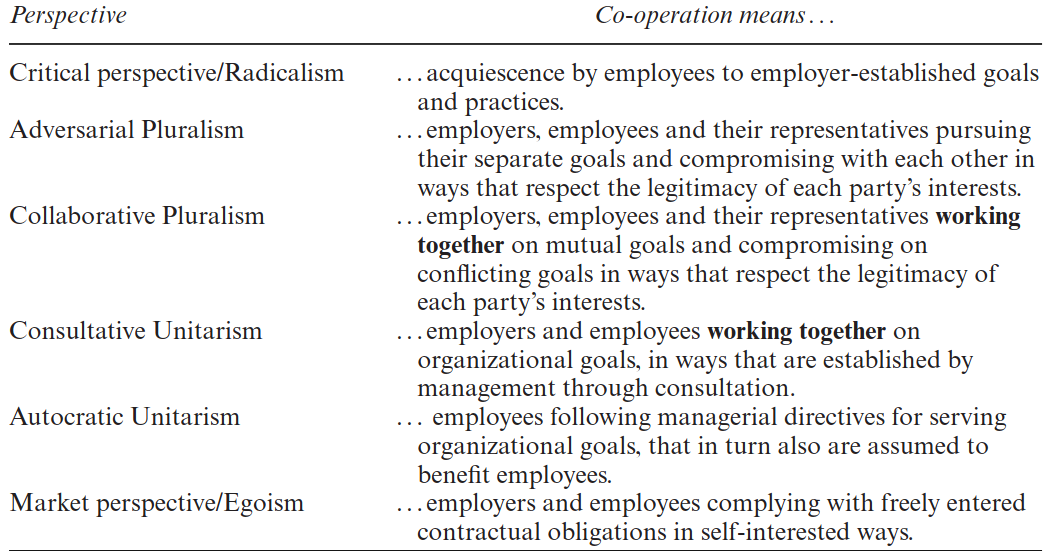
\includegraphics[width=0.6\textwidth]{
			CorporationPerspectives.png
		}
	\end{figure}

	\chapter{Kontrollskrivning 2}
	\newpage
	\section{Thylefors, I. (2019) Samarbete och konflikter}
	Konflikter, motsättningar och samarbetsproblem kommer att
	existera så länge som människor måste samverka. \textbf{Konflikt}
	= sammanstötning mellan olika intressen/krafter. \textbf{Mellanmänsklig
	konflikt} = all oenighet som vi investerar psykisk energi
	i (motsättningar som vi bryr oss om, som upptar oss). Två
	kategorier av konflikter: pseudokonflikter, verkliga
	konflikter. \textbf{Verkliga konflikter} = har
	substantiellt innehåll, ex oenighet om arbetsmetoder/verksamhetens
	framtida inriktning (lätt att göra begriplig för
	utomstående). \textbf{Pseudokonflikter} = skapas ur missnöje,
	har brett användningsområde (skapa dramatik som flykt undan
	vardaglig stress, leva ut allmänt missnöje, härska o söndra,
	skyla över andra mer hotande konflikter), kännetecknas av
	ovilja att verkligen komma till rätta med dem, funktion är att
	tangera \textbf{missförståndskonflikterna} (vanliga i arbetsgrupper
	med bristfällig information/kommunikation). \textbf{Konfliktbearbetning}
	= utgå från att kontrollera vad det är för missförstånd, få
	människor att prata så klaras missförstånd och verkliga motsättningar
	upp. \textbf{Interpersonella konflikter} = mellanmänskliga och
	de som uppfattas vid arbetsplatsrelationer. \textbf{Intrapersonella
	konflikter} = inre personliga, ex starka skuldkänslor
	inför egen aggressivitet, förmedlas mer eller mindre medvetet
	i form av ironi, pessimism och intriger, infekterar därefter
	samarbetet i arbetsgruppen - ju större självkännedom desto mindre
	risk att inre konflikter drabbar en arbetsgrupp. \textbf{Apersonella/systemkonflikter}
	= konflikter som ligger utanför oss, bottnar i företagets/organisationens
	struktur, mål, roller, arbetsorganisation,
	resursfördelning, förs in på den lokala arbetsplatsen genom
	motstridigheter, oklarheter och rigiditet (icke ändamålsenlig
	resursfördelning skapar konflikter mellan individer/grupper,
	otydliga mål tolkas olika mellan individer och
	grupperingar). Bör se systemet/organisationen som verktyg
	att förebygga onödiga konflikter i en verksamhet. \textbf{Kalla/dolda
	konflikter} = missnöje, indirekt aggresivitet, tystnad, negativt
	skvaller etc, kan diskuteras bakom stängda dörrar men ej
	med den/de som uppfattas som motparter, kan vara ovetande om
	konflikt och inga initiativ till en lösning. Existerar för
	att stärka liten grupp i gemensamt intresse mot en yttre
	fiende, rädsla för konflikter. \textbf{Öppna/varma
	konflikter} = lätt att observera konflikter på arbetsplatser
	med öppen atmosfär (bråk, kritik, argument etc). \textbf{Alturistiska/osjälviska
	konflikter} = relaterade till målsättning och arbete,
	omsorg om andras intressen och rättigheter. Större förutsättningar
	att lösas konstruktivt. \textbf{Egoistiska konflikter} = orsakas
	av personliga behov och intressen, hantering kräver att
	någon med legitim makt (chef) går in och avgör tvisten. \textbf{Integrativ/vinna-vinna
	konflikter} = handlar om ömsesidiga eftergifter/vinster, alla
	parter ska bli vinnare, svårt att nå dessa lösningar. \textbf{Distributiva/vinna-förlora
	konflikter} =. \textbf{Värderingskonflikter (etik/moral)}
	= medvetenhet om etiska konsekvenser av val av teknik/företagsetablering/handelskontakter
	etc ger upphov till konflikter. Svårhanterliga pga ej går att
	förhandla/kompromissa om värderingar. Ett problem för den
	enskilde att ta ställning till. \textbf{Person/sakkonflikter}
	= olika åsikter, beteenden, handlingar, (sak och person) hänger
	ihop, svårt att se nyanser och att människor har för- o nackdelar.
	Mer uttalad tendens under stress att svart/vitmåla för att
	få en konsekvent bild. I arbetsgrupper bör man behandla alla
	på ett anständigt sätt oavsett åsikt om dem. \textbf{Konflikthantering}
	= avgör om konflikter blir konstruktiva/destruktiva för en arbetsenhet.
	Konflikter förutsättning för kreativitet, utveckling,
	förändring, uttalade motsättningar $\implies$ nytänkande + förbättring
	av förslag. \textbf{Homogenitet} = mindre variation i åsikter,
	färre konfliktanledningar.
	\begin{figure}[ht!]
		\begin{minipage}{.3\linewidth}
			\timage{1}{konfliktstilar.png}
		\end{minipage}
		\begin{minipage}{.7\linewidth}
			\textbf{Konfliktstil} = förhållningssätt i
			konfliktsituationer. 2-dimensionell modell, omsorg om
			andras intressen vs omsorg om egna intressen. Konfliktstilar
			ofta förvärvade under barndomen, används i varje
			situation: lönsamt att vara snäll $\implies$ anpassande
			strategi, dialog/ömsesidigt givande $\implies$
			gemensam problemlösning, konkurrens/tävlande $\implies$
			överlevnadsstrategi. \textbf{Situationsanpassad
			konflikthantering} = behöver välja olika strategier vid
			olika situationer. \textbf{Konflikttrappa} = olika faser
			i upptrappningen av en konflikt, visar att konflikter
			blir mer energikrävande allt eftersom de trappas upp, samt
			att konflikter som fångas upp i ett tidigt skede kan hanteras
			med begränsade insatser medan stora konflikter fordrar stora
			insatser. Steg 1 - det anas åsiktsskillnader i
			förhållande till något. Steg 2 - diskussionen börjar.
			Steg 3 - diskussionen leder till att skillnaderna
			kvarstår så parterna intar tydligare ståndpunkter och
			rustar för strid genom allianser. Steg 4 - parterna intar
			fasta positioner och går in för att vinna/förlora.
			Steg 5 - från att satsa på att vinna sakfrågan satsar
			man istället på att vinna över motståndaren.
		\end{minipage}
	\end{figure}
	\textbf{Kollektiva försvar} = används av grupper för att
	frysa/undvika konflikter, grupper utvecklar försvar för att
	skydda sig. Kollektiva coping-/anpassningsmekanismer framträder
	när belastningen ökar och klingar av när den minskar.
	\textbf{Gruppförsvararen} = vissa grupper förlägger inre konflikter
	till omvärlden, svetsas ihop gentemot omvärlden. \textbf{Grupptänkande}
	= massivt grupptryck som sätter det kritiska tänkandet ur
	spel, var o en ålägger självcensur + håller inne med motstridiga
	synpunkter. Vanligt i högstatusgrupper. \textbf{Problemlösning}
	= steg 1 försök ringa in vad motsättningen handlar om (fakta,
	mål, metoder, värderingar etc) och kan underlätta en lösning,
	har de inte tillgång på samma information kan mer
	information vara en lösning. Insikt om rollens betydelse kan
	avpersonifiera en konflikt och bidra till förståelse för olika
	perspektiv. Steg 2 - identifiera intressenter i konflikten,
	använd \textbf{de fyra v-frågorna} (vad,varför,var och vilka).
	Leta alternativa lösningsförslag, undersöka konsekvenserna
	av dem, ta fram överenskommelse som följs upp. Systematisk
	analys av en konflikt ger struktur som fångar upp den del
	av den osäkerhet och obehag som försvårar en bearbetning (kan
	kritiseras (Edward de Bono) av uppehålla sig vid hinder och
	problem istället för möjligheter, rekommendation är att
	försöka lyfta sig från aktuellt problem genom fokus på vad
	man vill uppnå). \textbf{Förebygga konflikter} = skapa en tydlig/konsekvent
	struktur i form av ramar, arbets- och befattningsbeskrivningar
	och målformuleringar. Finna den optimala graden av likhet
	för varje verksamhet (likhet minskar konfliktanledningar men
	ökar risk för stagnation). Arbetsfördelning som separerar antagonister
	från varandra och normutveckling för att undvika kontroversiella
	ämnen behåller god stämning.
\end{document}